\documentclass[11pt]{article}

\usepackage[margin=1in]{geometry}
\usepackage{amsmath,amssymb,mathtools}
\usepackage{booktabs}
\usepackage{enumitem}
\usepackage{graphicx}
\usepackage{tikz}
\usetikzlibrary{arrows.meta,calc,positioning}
\usepackage{hyperref}
\usepackage{microtype}
\usepackage{xcolor}

\hypersetup{colorlinks=true,linkcolor=blue,urlcolor=blue}
\allowdisplaybreaks

\newcommand{\R}{\mathbb R}
\newcommand{\E}{\mathbb E}
\newcommand{\N}{\mathcal N}
\newcommand{\dd}{\,\mathrm d}

\title{A First-Year-University Explainer For Standard-Normal GHQ, SGQF Levels, Tensor Labels, Sparse-Grid Level, And Smolyak Construction}
\author{Chak Wong}
\date{2026-06-09}

\begin{document}
\maketitle

\begin{abstract}
This note is written for a reader who keeps seeing phrases such as
``level-2 rule,'' ``tensor rule \((2,2)\),'' ``sparse-grid level \(L=2\),'' and
``Smolyak construction,'' but does not yet feel that those phrases mean
something concrete.  The goal is not to present new theory.  The goal is to
explain, slowly and with explicit examples, what those phrases mean in the
sparse-grid quadrature filtering material based on Jia, Xin, and Cheng.  The
central message is simple: the same word ``level'' is being used for different
jobs.  A one-dimensional rule level labels a rule family member such as \(I_1\)
or \(I_2\).  A tensor label such as \((2,2)\) says which one-dimensional level
is used in each coordinate.  A sparse-grid level such as \(L=2\) says which
tensor rules are allowed into the sparse-grid approximation.  Smolyak
construction means: take several tensor rules, attach plus or minus coefficients
to them, and merge repeated point contributions.  Those are related ideas, but
they are not the same idea.
\end{abstract}

\tableofcontents

\section{If you remember only six sentences}
\label{sec:six-sentences}

If the rest of the note feels long, keep these six sentences in mind.
\begin{enumerate}[leftmargin=0.28in]
  \item A rule such as \(I_1\), \(I_2\), or \(I_3\) is a \emph{one-dimensional}
  weighted-average recipe for approximating a Gaussian integral.
  \item In BayesFilter's default convention, these one-dimensional rules come
  from standard-normal Gauss--Hermite quadrature, abbreviated standard-normal
  GHQ.
  \item A label such as \((2,1)\) or \((2,2,2)\) says: use one rule level in
  each coordinate, then take the Cartesian product.
  \item A sparse-grid level such as \(L=2\) does \emph{not} mean the same thing
  as the tensor label \((2,2)\) or \((2,2,2)\).
  \item Smolyak construction means: take several tensor rules, attach plus or
  minus coefficients to them, add them together, and merge repeated points.
  \item The numbers 1, 2, 3 in these labels are not polynomial degrees.  They
  are level labels, and the source paper ties level \(\ell\) to exactness of at
  least degree \(2\ell-1\) in one dimension \cite{jia2012sparsegrid}.
\end{enumerate}

\section{What are we trying to approximate?}
\label{sec:basic-goal}

Before discussing sparse grids, it helps to remember the original problem.  We
want to approximate a Gaussian integral such as
\begin{equation}
  \int_{\R} \psi(\xi)\,\phi(\xi)\,\dd\xi,
  \qquad
  \phi(\xi)=\frac{1}{\sqrt{2\pi}}e^{-\xi^2/2}.
  \label{eq:basic-gaussian-integral}
\end{equation}
The function \(\phi\) is the standard-normal density.  The function \(\psi\) is
whatever function we want to average.

A quadrature rule replaces the integral by a weighted sum:
\begin{equation}
  I_\ell[\psi]
  =
  \sum_{a=1}^{s_\ell}\omega_{\ell,a}\,\psi(\zeta_{\ell,a}).
  \label{eq:generic-1d-rule}
\end{equation}
Here:
\begin{itemize}[leftmargin=0.28in]
  \item \(\zeta_{\ell,a}\) are the nodes, meaning the places where we evaluate
  \(\psi\),
  \item \(\omega_{\ell,a}\) are the weights, meaning how much each evaluation
  counts,
  \item \(s_\ell\) is the number of nodes used by level \(\ell\).
\end{itemize}

So a one-dimensional rule level is simply a particular weighted-average recipe.

\section{What is standard-normal GHQ?}
\label{sec:standard-normal-ghq}

This is one of the things that should be stated more explicitly.

\subsection{Plain-English meaning}

GHQ stands for \emph{Gauss--Hermite quadrature}.  In the BayesFilter chapter, the
default family of one-dimensional rules is the standard-normal GHQ family.

You do \emph{not} need to know Hermite polynomials to read the note.  For our
purposes, you only need to know this:
\begin{quote}
standard-normal GHQ means a precomputed list of nodes and weights designed to
approximate integrals against the standard-normal density \(\phi(\xi)\).
\end{quote}

\subsection{BayesFilter default family}

The BayesFilter chapter fixes the default family as
\begin{equation}
  I_\ell = \textsc{OneDimGHQ}(2\ell-1).
  \label{eq:ghq-family-policy}
\end{equation}
This means:
\begin{itemize}[leftmargin=0.28in]
  \item level 1 uses a 1-point standard-normal GHQ rule,
  \item level 2 uses a 3-point standard-normal GHQ rule,
  \item level 3 uses a 5-point standard-normal GHQ rule,
  \item in general, level \(\ell\) uses a \((2\ell-1)\)-point standard-normal GHQ
  rule.
\end{itemize}

So in BayesFilter the family is not mysterious:
\begin{equation}
  I_1, I_2, I_3, \ldots
  \quad\text{means}\quad
  \text{1-point, 3-point, 5-point, \ldots standard-normal GHQ rules.}
  \label{eq:ghq-family-plain-english}
\end{equation}

\subsection{Concrete low-level members}

The first two members are the ones used repeatedly in the teaching note.

\paragraph{Level 1.}
The level-1 rule is
\begin{equation}
  I_1:(0,1).
  \label{eq:I1-definition}
\end{equation}
This means: evaluate only at the center point 0 and give it full weight 1.  So
\begin{equation}
  I_1[\psi]=\psi(0).
  \label{eq:I1-action}
\end{equation}

\paragraph{Level 2.}
The level-2 rule is the familiar 3-point standard-normal GHQ rule
\begin{equation}
  I_2:
  \left\{\left(-\sqrt3,\frac16\right),\left(0,\frac23\right),
  \left(\sqrt3,\frac16\right)\right\}.
  \label{eq:I2-definition}
\end{equation}
This means
\begin{equation}
  I_2[\psi]
  =
  \frac16\psi(-\sqrt3)+\frac23\psi(0)+\frac16\psi(\sqrt3).
  \label{eq:I2-action}
\end{equation}

\paragraph{Level 3.}
Level 3 means: use the 5-point standard-normal GHQ rule.  The original teaching
note does not write out those five nodes and weights explicitly, but under the
BayesFilter default policy level 3 means ``the 5-point standard-normal GHQ
member of the same family.''

\subsection{Why the level number is not a polynomial degree}

The label ``2'' in \(I_2\) is a family label, not the degree of a polynomial.
For the concrete rule \eqref{eq:I2-definition}, one can check
\begin{align}
  I_2[1] &= 1,
  \label{eq:I2-const}\\
  I_2[\xi^2] &= \frac16(3)+\frac23(0)+\frac16(3)=1,
  \label{eq:I2-second}\\
  I_2[\xi^4] &= \frac16(9)+\frac23(0)+\frac16(9)=3.
  \label{eq:I2-fourth}
\end{align}
Because the rule is symmetric, odd powers cancel automatically:
\begin{equation}
  I_2[\xi]=I_2[\xi^3]=I_2[\xi^5]=0.
  \label{eq:I2-odd}
\end{equation}
So the specific 3-point rule called \(I_2\) is exact through degree 5 under the
standard-normal weight.  That is why ``level 2'' cannot mean ``degree 2.''

\section{What does the function symbol mean?}
\label{sec:what-is-F}

Another thing that easily feels too abstract is the symbol \(F\).

\subsection{Plain-English meaning}

When we write
\begin{equation}
  I_{\mathbf i}[F]
  \qquad\text{or}\qquad
  A_{b,L}[F],
  \label{eq:F-symbol-reading}
\end{equation}
we mean:
\begin{quote}
apply the quadrature rule to the function \(F\).
\end{quote}
So \(F\) is just the function we want to average under the Gaussian weight.

In one dimension I often wrote \(\psi\).  In several dimensions I switch to
\(F\).  They play the same role.

\subsection{Concrete example used later}

To make everything concrete, later we will use the three-variable function
\begin{equation}
  F(\xi_1,\xi_2,\xi_3)=e^{\xi_1\xi_2\xi_3}.
  \label{eq:main-example-function}
\end{equation}
This is a good teaching example because:
\begin{itemize}[leftmargin=0.28in]
  \item it is clearly nonlinear,
  \item it depends on all three variables together,
  \item if any one coordinate is 0, then the product \(\xi_1\xi_2\xi_3\) becomes
  0 and \(F=1\),
  \item but at the full three-way corner points \((\pm\sqrt3,\pm\sqrt3,\pm\sqrt3)\)
  the function is not 1.
\end{itemize}
That makes it ideal for seeing what a low sparse-grid level can and cannot see.

\section{The three jobs done by the word ``level''}
\label{sec:three-jobs}

This section is the heart of the note.  It separates the three jobs as clearly
as possible.

\subsection{Job 1: level of a one-dimensional rule}

The notation \(I_\ell\) means:
\begin{quote}
``the one-dimensional quadrature rule at level \(\ell\).''
\end{quote}
This is a one-dimensional object.

\subsection{Job 2: level inside a tensor label}

The notation
\[
  \mathbf i=(i_1,\ldots,i_b)
\]
means:
\begin{quote}
``in coordinate 1 use level \(i_1\), in coordinate 2 use level \(i_2\), and so
on.''
\end{quote}
So a tensor label such as \((2,1)\) is not a new kind of level.  It is just a
short way to list which one-dimensional rule level is used in each coordinate.

\subsection{Job 3: sparse-grid level}

The notation \(L\) in the sparse-grid rule means something different again.  It
controls which tensor rules are allowed into the sparse-grid approximation.

So when you see
\[
  L=2,
\]
you should hear:
\begin{quote}
``use the sparse-grid combination rule at level 2.''
\end{quote}
You should \emph{not} hear:
\begin{quote}
``keep the full tensor rule \((2,2)\)'' or ``keep the full tensor rule
\((2,2,2)\).''
\end{quote}

\subsection{One-line dictionary}

Here is the shortest useful dictionary:
\begin{align*}
  I_2 &:\ \text{one-dimensional rule},\\
  (2,2) &:\ \text{two-dimensional tensor label},\\
  (2,2,2) &:\ \text{three-dimensional tensor label},\\
  L=2 &:\ \text{sparse-grid combination level}.
\end{align*}
These symbols are related, but they are not interchangeable.

\section{Tensor labels explained slowly}
\label{sec:tensor-labels}

Suppose we move from one variable \(\xi\) to two variables \((\xi_1,\xi_2)\).
Now we can choose one one-dimensional rule for the first coordinate and one for
the second coordinate.

The multi-index
\[
  \mathbf i=(i_1,i_2)
\]
records those choices.

\subsection{What \texorpdfstring{\((1,1)\)}{(1,1)} means}

The label \((1,1)\) means:
\begin{quote}
use \(I_1\) in coordinate 1 and \(I_1\) in coordinate 2.
\end{quote}
Because each \(I_1\) has only one point, the tensor product has only one point:
\begin{equation}
  (0,0)
  \qquad\text{with weight}\qquad 1.
  \label{eq:tensor-11}
\end{equation}
So for any two-variable function \(F\),
\begin{equation}
  I_{(1,1)}[F]=F(0,0).
  \label{eq:I11-of-F}
\end{equation}

\subsection{What \texorpdfstring{\((1,2)\)}{(1,2)} means}

The label \((1,2)\) means:
\begin{quote}
use \(I_1\) in coordinate 1 and \(I_2\) in coordinate 2.
\end{quote}
So the first coordinate stays fixed at 0, while the second coordinate uses the
three points of \(I_2\).  Therefore the tensor points are
\begin{equation}
  (0,-\sqrt3),\qquad (0,0),\qquad (0,\sqrt3),
  \label{eq:tensor-12-points}
\end{equation}
with weights
\begin{equation}
  \frac16,\qquad \frac23,\qquad \frac16.
  \label{eq:tensor-12-weights}
\end{equation}
So
\begin{equation}
  I_{(1,2)}[F]
  =
  \frac16F(0,-\sqrt3)+\frac23F(0,0)+\frac16F(0,\sqrt3).
  \label{eq:I12-of-F}
\end{equation}

\subsection{What \texorpdfstring{\((2,1)\)}{(2,1)} means}

The label \((2,1)\) means:
\begin{quote}
use \(I_2\) in coordinate 1 and \(I_1\) in coordinate 2.
\end{quote}
So now the second coordinate stays fixed at 0, while the first coordinate uses
the three points of \(I_2\).  Therefore the tensor points are
\begin{equation}
  (-\sqrt3,0),\qquad (0,0),\qquad (\sqrt3,0),
  \label{eq:tensor-21-points}
\end{equation}
with the same weights
\begin{equation}
  \frac16,\qquad \frac23,\qquad \frac16.
  \label{eq:tensor-21-weights}
\end{equation}

\subsection{What \texorpdfstring{\((2,2)\)}{(2,2)} means}

The label \((2,2)\) means:
\begin{quote}
use \(I_2\) in coordinate 1 and \(I_2\) in coordinate 2.
\end{quote}
Because each coordinate contributes three points, the full tensor product has
\begin{equation}
  3\times 3=9
  \label{eq:nine-points-count}
\end{equation}
points:
\begin{align}
  &(-\sqrt3,-\sqrt3),\ (-\sqrt3,0),\ (-\sqrt3,\sqrt3),\nonumber\\
  &(0,-\sqrt3),\ (0,0),\ (0,\sqrt3),\nonumber\\
  &(\sqrt3,-\sqrt3),\ (\sqrt3,0),\ (\sqrt3,\sqrt3).
  \label{eq:nine-point-grid}
\end{align}

\paragraph{Very important warning.}
The tensor label \((2,2)\) does \emph{not} mean sparse-grid level 2.  It only
means ``use \(I_2\) in both coordinates.''

\section{The local index \texorpdfstring{\(\alpha\)}{alpha}: which actual point did you choose?}
\label{sec:alpha}

After choosing the tensor label \(\mathbf i\), we still need to choose a
particular point inside that tensor rule.  That is what the local index
\(\alpha\) does.

The general formulas are
\begin{align}
  \xi^{\mathbf i,\alpha}
  &=
  (\zeta_{i_1,\alpha_1},\ldots,\zeta_{i_b,\alpha_b}),
  \label{eq:xi-i-alpha}\\
  w^{\mathbf i,\alpha}
  &=
  \prod_{j=1}^b\omega_{i_j,\alpha_j}.
  \label{eq:w-i-alpha}
\end{align}

In beginner language:
\begin{quote}
\(\mathbf i\) chooses the rule level in each coordinate, while \(\alpha\) chooses
one actual node from inside those already-chosen rules.
\end{quote}

\section{What is sparse-grid level?}
\label{sec:what-is-sparse-grid-level}

Now we come to the first of your two direct questions.

\subsection{First plain-English answer}

Sparse-grid level tells us:
\begin{quote}
which tensor rules are allowed to participate in the sparse-grid approximation.
\end{quote}
It is a choice about the combination rule, not a choice about one particular
coordinatewise tensor rule.

\subsection{The formal active band}

The teaching note uses the active band
\begin{equation}
  \mathcal A_{b,L}
  =
  \{\mathbf i\in\mathbb N^b: L\le |\mathbf i|\le L+b-1\},
  \qquad
  |\mathbf i|=i_1+\cdots+i_b.
  \label{eq:active-band}
\end{equation}
This says:
\begin{quote}
if the total index of a tensor label \(\mathbf i\) lies between \(L\) and
\(L+b-1\), then that tensor rule is allowed into the sparse-grid construction.
\end{quote}

\subsection{Two-dimensional example: sparse-grid level \texorpdfstring{\(L=2\)}{L=2}}

Take
\[
  b=2,
  \qquad
  L=2.
\]
Then the active-band condition becomes
\[
  2\le |\mathbf i|\le 3.
\]
So the allowed tensor labels are exactly
\begin{equation}
  (1,1),\qquad (1,2),\qquad (2,1).
  \label{eq:2d-active-rules}
\end{equation}
The tensor label \((2,2)\) is not allowed, because
\begin{equation}
  |(2,2)|=4,
  \qquad
  4\notin [2,3].
  \label{eq:22-not-active}
\end{equation}
So sparse-grid level 2 in two dimensions does not mean ``use \((2,2)\).''
Instead it means ``use the tensor rules whose total level lies in the allowed
band for \(L=2\).''

\subsection{Three-dimensional example: sparse-grid level \texorpdfstring{\(L=2\)}{L=2}}

Take
\[
  b=3,
  \qquad
  L=2.
\]
Then the active-band condition becomes
\[
  2\le |\mathbf i|\le 4.
\]
Because each coordinate level is at least 1, the allowed tensor labels are
\begin{equation}
  (1,1,1),\qquad (1,1,2),\qquad (1,2,1),\qquad (2,1,1).
  \label{eq:3d-active-rules-level-section}
\end{equation}
Again, the full tensor label \((2,2,2)\) is not allowed, because
\begin{equation}
  |(2,2,2)|=6,
  \qquad
  6\notin [2,4].
  \label{eq:222-not-active}
\end{equation}

\paragraph{Plain-language summary.}
Sparse-grid level does not tell us which one-dimensional rule is used in every
coordinate.  It tells us which \emph{multi-coordinate tensor rules} are admitted
into the sparse approximation.

\section{What is Smolyak construction?}
\label{sec:what-is-smolyak}

Now we come to the second direct question.

\subsection{First plain-English answer}

Smolyak construction means:
\begin{quote}
start with several tensor rules, attach plus or minus coefficients to them, add
them together, and merge repeated points.
\end{quote}

This is the key idea.  Smolyak is not just ``throw away some tensor points.''
Smolyak is a signed combination of whole tensor rules.

\subsection{The formal formula}

The teaching note writes the sparse-grid rule as
\begin{equation}
  A_{b,L}[F]
  =
  \sum_{\mathbf i\in\mathcal A_{b,L}} c_{\mathbf i} I_{\mathbf i}[F],
  \label{eq:smolyak-formula}
\end{equation}
where the coefficients are
\begin{equation}
  c_{\mathbf i}
  =
  (-1)^{L+b-1-|\mathbf i|}
  \binom{b-1}{L+b-1-|\mathbf i|}.
  \label{eq:smolyak-coefficients}
\end{equation}
If that formula looks frightening, the beginner message is much simpler:
\begin{quote}
Smolyak tells us which tensor rules to combine and whether each one enters with
plus sign or minus sign.
\end{quote}

\section{What does it mean that tensor rules are combined by Smolyak?}
\label{sec:combined-by-smolyak}

This is the question that usually needs the most concrete explanation.

\subsection{First understand what one tensor rule is}

A tensor rule such as \((1,2)\) is already a list of points and weights.
Another tensor rule such as \((2,1)\) is another list of points and weights.
The Smolyak construction does not choose one of them and discard the others.
Instead it says:
\begin{quote}
add together the weighted sums from several tensor rules.
\end{quote}

So when we say
\begin{equation}
  A_{2,2}[F] = -I_{(1,1)}[F] + I_{(1,2)}[F] + I_{(2,1)}[F],
  \label{eq:2d-smolyak}
\end{equation}
we mean:
\begin{enumerate}[leftmargin=0.28in]
  \item evaluate \(F\) on the tensor rule \((1,1)\),
  \item evaluate \(F\) on the tensor rule \((1,2)\),
  \item evaluate \(F\) on the tensor rule \((2,1)\),
  \item subtract the first weighted sum,
  \item add the second weighted sum,
  \item add the third weighted sum.
\end{enumerate}
That is what it means to say that the tensor rules are combined by Smolyak.

\subsection{Concrete two-dimensional example, step by step}

Take the one-dimensional rules
\begin{equation}
  I_1:(0,1),
  \qquad
  I_2:
  \left\{\left(-\sqrt3,\frac16\right),\left(0,\frac23\right),
  \left(\sqrt3,\frac16\right)\right\}.
  \label{eq:2d-univariate-rules}
\end{equation}
For sparse-grid level \(L=2\) in dimension \(b=2\), the active tensor rules are
\((1,1)\), \((1,2)\), and \((2,1)\).  Their tensor points are:
\begin{align}
  (1,1) &: \{(0,0)\},
  \label{eq:rule11-set}\\
  (1,2) &: \{(0,-\sqrt3),(0,0),(0,\sqrt3)\},
  \label{eq:rule12-set}\\
  (2,1) &: \{(-\sqrt3,0),(0,0),(\sqrt3,0)\}.
  \label{eq:rule21-set}
\end{align}
The Smolyak coefficients are
\begin{equation}
  c_{(1,1)}=-1,
  \qquad
  c_{(1,2)}=1,
  \qquad
  c_{(2,1)}=1.
  \label{eq:2d-smolyak-coeffs}
\end{equation}
So the combined rule is exactly
\begin{equation}
  A_{2,2}[F] = -I_{(1,1)}[F] + I_{(1,2)}[F] + I_{(2,1)}[F].
  \label{eq:2d-smolyak-repeat}
\end{equation}

Now let us combine the point contributions one by one.

\paragraph{Contribution from \texorpdfstring{\((1,1)\)}{(1,1)}.}
This rule contributes only the center point:
\[
  (0,0) \quad\text{with signed weight}\quad -1.
\]

\paragraph{Contribution from \texorpdfstring{\((1,2)\)}{(1,2)}.}
This contributes
\[
  (0,-\sqrt3),\ (0,0),\ (0,\sqrt3)
\]
with signed weights
\[
  \frac16,\ \frac23,\ \frac16.
\]

\paragraph{Contribution from \texorpdfstring{\((2,1)\)}{(2,1)}.}
This contributes
\[
  (-\sqrt3,0),\ (0,0),\ (\sqrt3,0)
\]
with signed weights
\[
  \frac16,\ \frac23,\ \frac16.
\]

\subsection{Now merge the repeated points}

The point \((0,0)\) appears in all three tensor rules.  So its final weight is
obtained by adding its three signed contributions:
\begin{equation}
  -1+\frac23+\frac23=\frac13.
  \label{eq:center-weight-2d}
\end{equation}
The four axis points each appear only once, so they each keep weight \(1/6\).
Therefore the final merged sparse-grid cloud is
\begin{equation}
  (0,0),\quad (\pm\sqrt3,0),\quad (0,\pm\sqrt3),
  \label{eq:five-point-cloud}
\end{equation}
with weights
\begin{equation}
  \frac13,\quad \frac16,\quad \frac16,\quad \frac16,\quad \frac16.
  \label{eq:five-point-weights}
\end{equation}

\paragraph{Why this cloud should remind you of a UKF picture.}
A beginner who has seen a UKF or Unscented Transform diagram should notice that
this merged SGQF cloud looks familiar: there is one center point and several
symmetric off-center points.  That visual similarity is real and useful.  Both
constructions use a deterministic weighted point cloud to approximate Gaussian
expectations.  However, the final SGQF cloud was not chosen all at once by one
sigma-point formula.  It was built by combining the tensor rules \((1,1)\),
\((1,2)\), and \((2,1)\) with Smolyak coefficients and then merging repeated
points.

\begin{figure}[htbp]
\centering
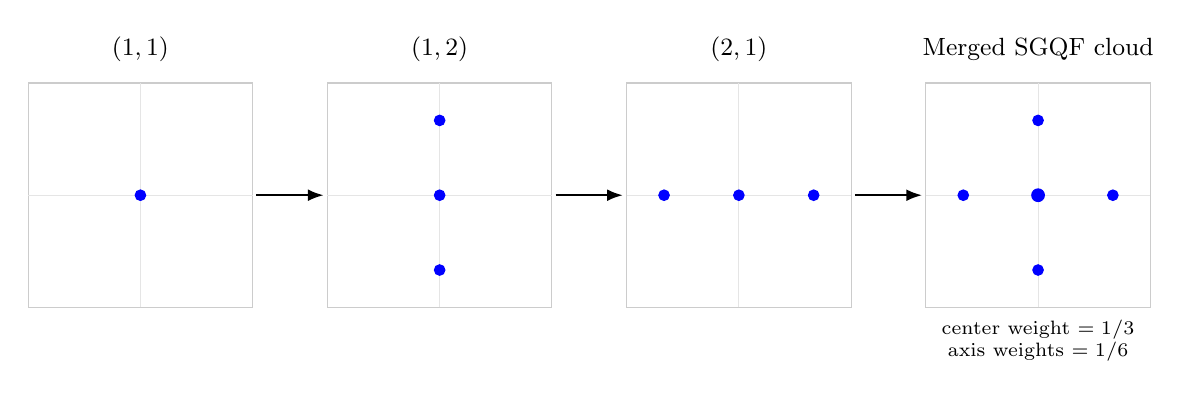
\begin{tikzpicture}[scale=0.95, every node/.style={font=\small}]
  \def\sep{4.0}
  \begin{scope}[shift={(0,0)}]
    \draw[gray!40] (-1.5,-1.5) rectangle (1.5,1.5);
    \draw[gray!20] (-1.5,0) -- (1.5,0);
    \draw[gray!20] (0,-1.5) -- (0,1.5);
    \node[align=center] at (0,1.95) {$(1,1)$};
  \end{scope}
  \begin{scope}[shift={(\sep,0)}]
    \draw[gray!40] (-1.5,-1.5) rectangle (1.5,1.5);
    \draw[gray!20] (-1.5,0) -- (1.5,0);
    \draw[gray!20] (0,-1.5) -- (0,1.5);
    \node[align=center] at (0,1.95) {$(1,2)$};
  \end{scope}
  \begin{scope}[shift={(2*\sep,0)}]
    \draw[gray!40] (-1.5,-1.5) rectangle (1.5,1.5);
    \draw[gray!20] (-1.5,0) -- (1.5,0);
    \draw[gray!20] (0,-1.5) -- (0,1.5);
    \node[align=center] at (0,1.95) {$(2,1)$};
  \end{scope}
  \begin{scope}[shift={(3*\sep,0)}]
    \draw[gray!40] (-1.5,-1.5) rectangle (1.5,1.5);
    \draw[gray!20] (-1.5,0) -- (1.5,0);
    \draw[gray!20] (0,-1.5) -- (0,1.5);
    \node[align=center] at (0,1.95) {Merged SGQF cloud};
  \end{scope}
  % panel 1
  \filldraw[blue] (0,0) circle (2pt);
  % panel 2
  \begin{scope}[shift={(\sep,0)}]
    \filldraw[blue] (0,0) circle (2pt);
    \filldraw[blue] (0,1) circle (2pt);
    \filldraw[blue] (0,-1) circle (2pt);
  \end{scope}
  % panel 3
  \begin{scope}[shift={(2*\sep,0)}]
    \filldraw[blue] (0,0) circle (2pt);
    \filldraw[blue] (1,0) circle (2pt);
    \filldraw[blue] (-1,0) circle (2pt);
  \end{scope}
  % panel 4
  \begin{scope}[shift={(3*\sep,0)}]
    \filldraw[blue] (0,0) circle (2.4pt);
    \filldraw[blue] (1,0) circle (2pt);
    \filldraw[blue] (-1,0) circle (2pt);
    \filldraw[blue] (0,1) circle (2pt);
    \filldraw[blue] (0,-1) circle (2pt);
    \node[align=center, font=\scriptsize] at (0,-1.95) {center weight $=1/3$\\axis weights $=1/6$};
  \end{scope}
  % arrows
  \draw[-{Latex[length=2mm]}, thick] (1.55,0) -- (2.45,0);
  \draw[-{Latex[length=2mm]}, thick] (5.55,0) -- (6.45,0);
  \draw[-{Latex[length=2mm]}, thick] (9.55,0) -- (10.45,0);
\end{tikzpicture}
\caption{How the two-dimensional SGQF cloud is built: the active tensor rules
\((1,1)\), \((1,2)\), and \((2,1)\) are combined, and repeated point
contributions are merged.  The final five-point cloud has the kind of central
plus symmetric off-center geometry that may remind a reader of a UKF picture,
but its construction rule is different.}
\label{fig:sgqf-cloud-buildup}
\end{figure}

\paragraph{A direct visual comparison with a UKF-style sketch.}
The next picture makes the similarity and difference explicit.  The left panel is
the merged SGQF cloud from Figure~\ref{fig:sgqf-cloud-buildup}.  The right panel
is a canonical introductory UKF-style sigma-point sketch: one center point plus
four symmetric axis points.  The pictures look similar because both methods are
deterministic weighted point clouds for Gaussian expectations.  But the SGQF
cloud comes from active tensor-rule selection and Smolyak recombination, whereas
a UKF picture is usually presented as one directly specified sigma-point set.

\begin{figure}[htbp]
\centering
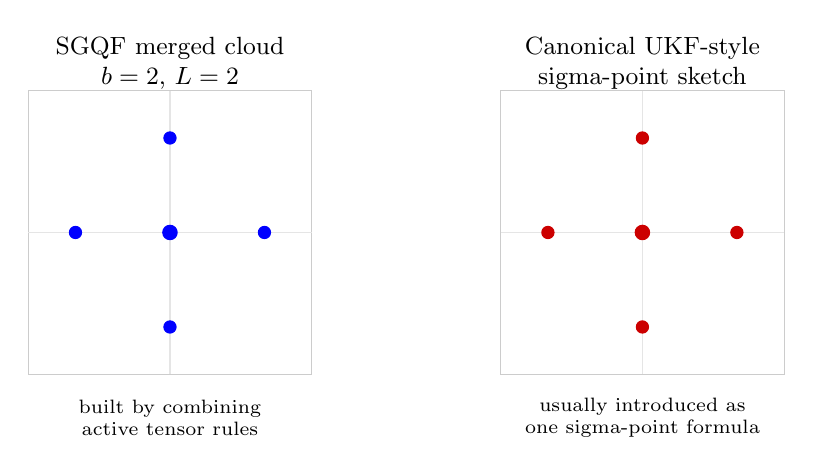
\begin{tikzpicture}[scale=1.0, every node/.style={font=\small}]
  % left panel SGQF
  \begin{scope}[shift={(0,0)}]
    \draw[gray!40] (-1.8,-1.8) rectangle (1.8,1.8);
    \draw[gray!20] (-1.8,0) -- (1.8,0);
    \draw[gray!20] (0,-1.8) -- (0,1.8);
    \node[align=center] at (0,2.15) {SGQF merged cloud\\$b=2$, $L=2$};
    \filldraw[blue] (0,0) circle (2.6pt);
    \filldraw[blue] (1.2,0) circle (2.2pt);
    \filldraw[blue] (-1.2,0) circle (2.2pt);
    \filldraw[blue] (0,1.2) circle (2.2pt);
    \filldraw[blue] (0,-1.2) circle (2.2pt);
    \node[font=\scriptsize, align=center] at (0,-2.35) {built by combining\\active tensor rules};
  \end{scope}
  % right panel UKF style
  \begin{scope}[shift={(6.0,0)}]
    \draw[gray!40] (-1.8,-1.8) rectangle (1.8,1.8);
    \draw[gray!20] (-1.8,0) -- (1.8,0);
    \draw[gray!20] (0,-1.8) -- (0,1.8);
    \node[align=center] at (0,2.15) {Canonical UKF-style\\sigma-point sketch};
    \filldraw[red!80!black] (0,0) circle (2.6pt);
    \filldraw[red!80!black] (1.2,0) circle (2.2pt);
    \filldraw[red!80!black] (-1.2,0) circle (2.2pt);
    \filldraw[red!80!black] (0,1.2) circle (2.2pt);
    \filldraw[red!80!black] (0,-1.2) circle (2.2pt);
    \node[font=\scriptsize, align=center] at (0,-2.35) {usually introduced as\\one sigma-point formula};
  \end{scope}
\end{tikzpicture}
\caption{A safe visual analogy.  The SGQF merged cloud and a canonical
introductory UKF-style sigma-point sketch can look similar geometrically: both
show a center point plus symmetric axis points.  The similarity is useful for
intuition, but the construction is different.}
\label{fig:sgqf-vs-ukf-2d}
\end{figure}

\section{How sparse-grid rules compare with UKF-style sigma-point filters}
\label{sec:ukf-comparison}

The user asked specifically about UKF.  That is the right comparison to make,
because the pictures can look similar while the construction logic is different.

\subsection{What is similar}

At the most basic visual and computational level, SGQF clouds and UKF-style
sigma-point sets have a real similarity:
\begin{itemize}[leftmargin=0.28in]
  \item both are deterministic weighted point clouds,
  \item both are used to approximate Gaussian expectations,
  \item both are centered around the Gaussian mean,
  \item both often show symmetry around that center,
  \item both can be drawn as ``center plus off-center points'' diagrams.
\end{itemize}
So it is completely reasonable for a beginner to think, ``this sparse-grid cloud
looks a bit like a UKF picture.''

\subsection{What is different in construction}

This is the most important difference.

\paragraph{Typical beginner picture of UKF.}
A UKF is usually introduced as one directly specified sigma-point set: choose one
formula for the sigma-point locations and one formula for the weights, then use
that single point cloud to approximate Gaussian expectations.

\paragraph{SGQF construction.}
SGQF is built more indirectly.  In the present note the construction is:
\begin{enumerate}[leftmargin=0.28in]
  \item choose a one-dimensional rule family such as standard-normal GHQ,
  \item choose a sparse-grid level \(L\),
  \item determine which tensor rules are active,
  \item attach Smolyak coefficients to those active tensor rules,
  \item merge repeated point contributions.
\end{enumerate}
So the final SGQF cloud is not usually chosen all at once by one sigma-point
formula.  It is assembled from several smaller tensor rules.

\subsection{What the source paper says about UKF}

The source-supported connection is narrower and more precise than ``SGQF is just
UKF.''  Jia, Xin, and Cheng show that the unscented-transform point set appears
as a level-2 sparse-grid member under the source's one-point and three-point
univariate choice.  So the right beginner conclusion is:
\begin{quote}
UKF and low-level SGQF live in the same broad family of deterministic Gaussian
point-set approximations, but SGQF is a more systematic sparse-grid construction,
not merely a relabeling of the UKF.
\end{quote}

\subsection{When the final cloud can look similar to a UKF cloud}

The user raised an important subtlety: if both SGQF and a UKF-style cloud are
trying to match the same second moments, should the weights become the same or at
least similar?  The answer is: sometimes yes, but not always.  Second-moment
accuracy by itself does not uniquely determine the whole point cloud.

To see this, imagine a symmetric axis cloud in dimension \(d\):
\begin{itemize}[leftmargin=0.28in]
  \item one center point at the origin with weight \(w_0\),
  \item two axis points \(\pm a e_i\) in each coordinate direction,
  \item every off-center point has the same weight \(w\).
\end{itemize}
There are therefore \(2d\) off-center points.

If we want the weights to sum to one, we need
\begin{equation}
  w_0 + 2dw = 1.
  \label{eq:axis-cloud-total-weight}
\end{equation}
If we want the cloud to reproduce variance 1 in each coordinate, then only the
pair \(+ae_i\) and \(-ae_i\) contributes to the second moment in that coordinate,
so we need
\begin{equation}
  2wa^2 = 1.
  \label{eq:axis-cloud-second-moment}
\end{equation}
From \eqref{eq:axis-cloud-second-moment} we get
\begin{equation}
  w = \frac{1}{2a^2},
  \qquad
  w_0 = 1-\frac{d}{a^2}.
  \label{eq:axis-cloud-weights-solved}
\end{equation}
So second-moment accuracy does not force one unique choice of weights.  It only
says that once the radius \(a\) is chosen, the weights are determined by that
radius.

\paragraph{Two-dimensional example.}
If \(d=2\) and \(a=\sqrt3\), then
\begin{equation}
  w = \frac{1}{2\cdot 3}=\frac16,
  \qquad
  w_0 = 1-\frac{2}{3}=\frac13.
  \label{eq:axis-cloud-2d-weights}
\end{equation}
So the resulting cloud has exactly the same weights as the merged two-dimensional
SGQF level-2 cloud:
\begin{equation}
  \text{center weight }=\frac13,
  \qquad
  \text{each axis weight }=\frac16.
  \label{eq:axis-cloud-2d-match}
\end{equation}
This is one reason the final SGQF picture can look very UKF-like.

\paragraph{Three-dimensional example.}
If \(d=3\) and again \(a=\sqrt3\), then
\begin{equation}
  w = \frac16,
  \qquad
  w_0 = 1-\frac{3}{3}=0.
  \label{eq:axis-cloud-3d-weights}
\end{equation}
So the center weight disappears and the six axis points each carry weight
\(1/6\).  This matches the low-level three-dimensional SGQF toy cloud in the
main note.

\paragraph{What this does and does not show.}
This calculation shows that if two methods end with the same symmetric axis
geometry and both enforce the same second-moment conditions, then the final
weights can indeed match.  But it does \emph{not} show that SGQF and UKF are the
same construction.  It only shows that the final low-level cloud can coincide in
special cases.

\subsection{Why sparse-grid level is not just ``point spread''}

A UKF is often introduced with parameters that directly control the final
sigma-point geometry or weighting.  By contrast, sparse-grid level \(L\) does not
simply say ``spread the same cloud farther out'' or ``keep the same pattern but
change one knob.''  Instead, sparse-grid level decides which tensor rules are
allowed into the active band.  The final cloud changes because the construction
includes different tensor components, not because one predeclared sigma-point set
was stretched.

\subsection{Why Smolyak is not ``delete a few points''}

A beginner might imagine that SGQF starts from a full tensor grid and then merely
deletes some inconvenient points.  That is not what Smolyak does.  Smolyak builds
a signed combination of whole tensor rules.  Some repeated points then merge, and
some weights can be reduced or canceled by adding signed contributions together.
So the final SGQF cloud is an algebraic recombination of tensor rules, not only a
pruned subset of a larger grid.

\subsection{The signed-weight difference}

This is another useful contrast with the usual beginner UKF picture.  In many
introductory sigma-point diagrams, readers imagine the weights as simple positive
masses attached to the points.  Smolyak construction is more subtle: it combines
tensor rules with signed coefficients.  After merging, some final weights may be
smaller than expected or even negative in other sparse-grid settings.  So an SGQF
cloud can resemble a sigma-point cloud geometrically while behaving differently
algebraically.

\subsection{Safe one-paragraph summary}

A good beginner summary is this.  A UKF-style sigma-point picture and a low-level
SGQF cloud can look similar because both are deterministic weighted point sets
used to approximate Gaussian expectations.  But the UKF picture is usually taught
as one directly specified sigma-point formula, whereas SGQF is built by choosing
one-dimensional rules, selecting active tensor rules through sparse-grid level,
and then combining those tensor rules by Smolyak coefficients.  So the geometry
may look familiar while the construction logic is different.

\section{How sparse-grid level and Smolyak fit together}
\label{sec:level-and-smolyak-fit}

These two ideas fit together as follows.

\subsection{Sparse-grid level chooses the active tensor rules}

The sparse-grid level \(L\) tells us which tensor rules belong to the active band
\(\mathcal A_{b,L}\).

\subsection{Smolyak tells us how to combine those active tensor rules}

Once the active tensor rules have been selected, the Smolyak formula tells us
what sign and coefficient each active tensor rule receives, and how their
contributions are added together.

\subsection{One-sentence summary}

If you want one sentence to remember, use this one:
\begin{quote}
The sparse-grid level chooses which tensor rules are active, and the Smolyak
construction tells us how to combine those active tensor rules into one sparse
rule.
\end{quote}

\section{A full worked three-dimensional example using \texorpdfstring{\(F(\xi_1,\xi_2,\xi_3)=e^{\xi_1\xi_2\xi_3}\)}{F(xi1,xi2,xi3)=exp(xi1 xi2 xi3)}}
\label{sec:full-3d-example}

Now let us put everything together in one explicit example.

\subsection{Step 1: choose the function}

Take
\begin{equation}
  F(\xi_1,\xi_2,\xi_3)=e^{\xi_1\xi_2\xi_3}.
  \label{eq:full-example-F}
\end{equation}
This means:
\begin{itemize}[leftmargin=0.28in]
  \item if one coordinate is 0, then \(F=1\),
  \item if all three coordinates are nonzero, then \(F\) may be much larger or
  much smaller than 1.
\end{itemize}

\subsection{Step 2: evaluate the simplest tensor rule \texorpdfstring{\((1,1,1)\)}{(1,1,1)}}

The tensor rule \((1,1,1)\) uses \(I_1\) in all three coordinates.  So there is
only one point:
\[
  (0,0,0).
\]
Therefore
\begin{equation}
  I_{(1,1,1)}[F]=F(0,0,0)=e^{0\cdot 0\cdot 0}=1.
  \label{eq:I111-example}
\end{equation}

\subsection{Step 3: evaluate the tensor rule \texorpdfstring{\((2,1,1)\)}{(2,1,1)}}

The tensor rule \((2,1,1)\) uses \(I_2\) in coordinate 1 and \(I_1\) in
coordinates 2 and 3.  So the tensor points are
\[
  (-\sqrt3,0,0),\qquad (0,0,0),\qquad (\sqrt3,0,0).
\]
At all three points we have \(\xi_2=0\) and \(\xi_3=0\), so
\[
  \xi_1\xi_2\xi_3=0,
  \qquad
  F=e^0=1.
\]
Therefore
\begin{equation}
  I_{(2,1,1)}[F]
  =
  \frac16(1)+\frac23(1)+\frac16(1)=1.
  \label{eq:I211-example}
\end{equation}
By the same reasoning,
\begin{equation}
  I_{(1,2,1)}[F]=1,
  \qquad
  I_{(1,1,2)}[F]=1.
  \label{eq:I121-I112-example}
\end{equation}

\subsection{Step 4: choose sparse-grid level \texorpdfstring{\(L=2\)}{L=2}}

Take dimension \(b=3\) and sparse-grid level \(L=2\).  The active tensor rules
are
\begin{equation}
  (1,1,1),\qquad (1,1,2),\qquad (1,2,1),\qquad (2,1,1).
  \label{eq:3d-active-rules-full-example}
\end{equation}
The Smolyak coefficients are
\begin{equation}
  c_{(1,1,1)}=-2,
  \qquad
  c_{(1,1,2)}=1,
  \qquad
  c_{(1,2,1)}=1,
  \qquad
  c_{(2,1,1)}=1.
  \label{eq:3d-smolyak-coeffs-example}
\end{equation}
Therefore
\begin{equation}
  A_{3,2}[F]
  =
  -2I_{(1,1,1)}[F]+I_{(1,1,2)}[F]+I_{(1,2,1)}[F]+I_{(2,1,1)}[F].
  \label{eq:A32-example}
\end{equation}
Using \eqref{eq:I111-example}, \eqref{eq:I211-example}, and
\eqref{eq:I121-I112-example}, we get
\begin{equation}
  A_{3,2}[F]
  =
  -2(1)+1+1+1=1.
  \label{eq:A32-example-value}
\end{equation}
So in this example the sparse-grid level-2 rule gives the value 1.

\subsection{Step 5: compare with the full tensor rule \texorpdfstring{\((2,2,2)\)}{(2,2,2)}}

Now compare this with the full tensor rule \((2,2,2)\).  This rule uses \(I_2\)
in all three coordinates, so it has
\begin{equation}
  3\times 3\times 3=27
  \label{eq:27-point-count}
\end{equation}
raw tensor-product points.

\begin{figure}[htbp]
\centering
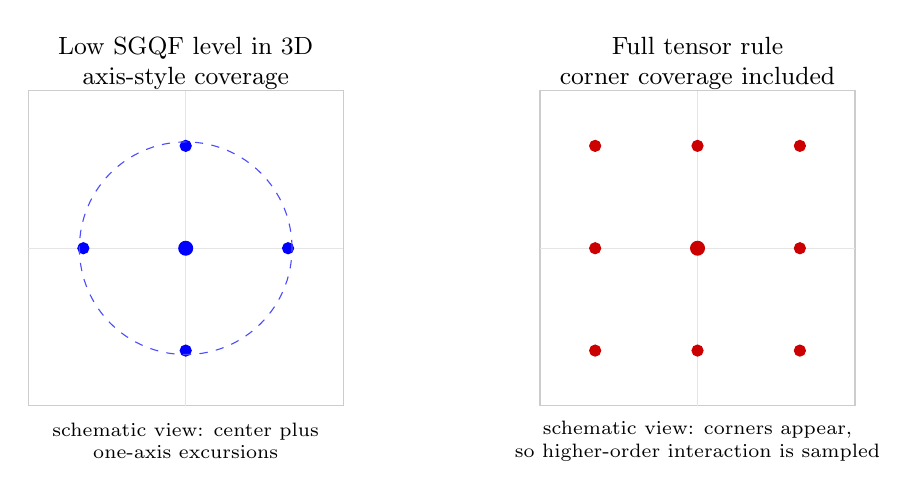
\begin{tikzpicture}[scale=1.0, every node/.style={font=\small}]
  % left: SGQF coverage
  \begin{scope}[shift={(0,0)}]
    \draw[gray!40] (-2,-2) rectangle (2,2);
    \draw[gray!20] (-2,0) -- (2,0);
    \draw[gray!20] (0,-2) -- (0,2);
    \node[align=center] at (0,2.35) {Low SGQF level in 3D\\axis-style coverage};
    \filldraw[blue] (0,0) circle (2.5pt);
    \filldraw[blue] (1.3,0) circle (2pt);
    \filldraw[blue] (-1.3,0) circle (2pt);
    \filldraw[blue] (0,1.3) circle (2pt);
    \filldraw[blue] (0,-1.3) circle (2pt);
    \draw[blue!70,dashed] (0,0) circle (1.35);
    \node[align=center, font=\scriptsize] at (0,-2.45) {schematic view: center plus\\one-axis excursions};
  \end{scope}
  % right: full tensor / corner coverage
  \begin{scope}[shift={(6.5,0)}]
    \draw[gray!40] (-2,-2) rectangle (2,2);
    \draw[gray!20] (-2,0) -- (2,0);
    \draw[gray!20] (0,-2) -- (0,2);
    \node[align=center] at (0,2.35) {Full tensor rule\\corner coverage included};
    \filldraw[red!80!black] (1.3,1.3) circle (2pt);
    \filldraw[red!80!black] (1.3,-1.3) circle (2pt);
    \filldraw[red!80!black] (-1.3,1.3) circle (2pt);
    \filldraw[red!80!black] (-1.3,-1.3) circle (2pt);
    \filldraw[red!80!black] (0,0) circle (2.5pt);
    \filldraw[red!80!black] (1.3,0) circle (2pt);
    \filldraw[red!80!black] (-1.3,0) circle (2pt);
    \filldraw[red!80!black] (0,1.3) circle (2pt);
    \filldraw[red!80!black] (0,-1.3) circle (2pt);
    \node[align=center, font=\scriptsize] at (0,-2.45) {schematic view: corners appear,\\so higher-order interaction is sampled};
  \end{scope}
\end{tikzpicture}
\caption{A schematic comparison for the three-variable example
$F(\xi_1,\xi_2,\xi_3)=e^{\xi_1\xi_2\xi_3}$.  A low sparse-grid level mainly sees
center and axis-type structure, while the full tensor rule also includes corner
coverage.  For a function driven by a genuine three-way product, those corners
matter.}
\label{fig:sgqf-vs-full-tensor-3d}
\end{figure}

Among those 27 points:
\begin{itemize}[leftmargin=0.28in]
  \item 19 points have at least one coordinate equal to 0, so at those points
  \(F=1\),
  \item 8 corner points have all coordinates equal to \(\pm\sqrt3\), so there
  \(\xi_1\xi_2\xi_3=\pm 3\sqrt3\) and
  \(F=e^{\pm 3\sqrt3}\).
\end{itemize}
Each corner weight is
\begin{equation}
  \frac16\cdot\frac16\cdot\frac16 = \frac1{216}.
  \label{eq:corner-weight}
\end{equation}
There are 4 positive-sign corners and 4 negative-sign corners, so
\begin{equation}
  I_{(2,2,2)}[F]
  =
  \frac{26}{27}+\frac{1}{54}e^{3\sqrt3}+\frac{1}{54}e^{-3\sqrt3}.
  \label{eq:I222-example}
\end{equation}
Numerically this is about
\begin{equation}
  I_{(2,2,2)}[F]\approx 4.32,
  \label{eq:I222-example-numeric}
\end{equation}
which is very different from the sparse-grid level-2 value
\(A_{3,2}[F]=1\).

\subsection{What this example teaches}

This example teaches something important and intuitive.

The function
\[
  F(\xi_1,\xi_2,\xi_3)=e^{\xi_1\xi_2\xi_3}
\]
contains a genuine three-way interaction because all three coordinates appear in
a product.  The low sparse-grid level \(L=2\) in three dimensions mainly uses the
center and one-axis rules.  Those points all have at least one zero coordinate,
so this low sparse-grid level cannot really see the full three-way corner
interaction.  By contrast, the full tensor rule \((2,2,2)\) does include the
corners, so it does see those large values.

So this single example shows how all the pieces fit together:
\begin{itemize}[leftmargin=0.28in]
  \item \(F\) is the function being integrated,
  \item \(I_1\) and \(I_2\) are one-dimensional GHQ rules,
  \item \((2,1,1)\) is a tensor label saying which 1D rule is used in each
  coordinate,
  \item sparse-grid level \(L=2\) chooses the active tensor rules,
  \item Smolyak tells us how to combine those active tensor rules,
  \item the final sparse-grid value can differ sharply from the full tensor value
  if the function depends strongly on interactions that the low sparse-grid level
  does not sample well.
\end{itemize}

\section{What does the source notation \texorpdfstring{\(N_q^b\)}{Nqb} mean?}
\label{sec:Nqb}

The source paper groups tensor labels by total index using
\begin{equation}
  N_q^b
  =
  \{\mathbf i=(i_1,\ldots,i_b)\in\mathbb N^b: i_1+\cdots+i_b=b+q\}.
  \label{eq:Nqb-definition}
\end{equation}
This looks abstract, but it is only a grouping device.

\subsection{Two-dimensional example}

If \(b=2\), then
\begin{align}
  N_0^2 &= \{(1,1)\},\\
  N_1^2 &= \{(1,2),(2,1)\},\\
  N_2^2 &= \{(1,3),(2,2),(3,1)\}.
\end{align}
So \(N_q^2\) simply groups tensor labels according to their total sum.

\subsection{Three-dimensional example}

If \(b=3\), then
\begin{align}
  N_0^3 &= \{(1,1,1)\},\\
  N_1^3 &= \{(1,1,2),(1,2,1),(2,1,1)\}.
\end{align}
Again, nothing mysterious is happening.  The set \(N_q^b\) is just organizing the
same tensor labels we already discussed.

\paragraph{Plain-language translation.}
When you see \(N_q^b\), read it as:
\begin{quote}
``the set of all tensor labels in \(b\) dimensions whose total index is
\(b+q\).''
\end{quote}

\section{What the source paper means by exactness levels}
\label{sec:exactness-levels}

The Jia--Xin--Cheng paper gives the following rule of thumb for the univariate
family.  A one-dimensional rule at level \(\ell\) is chosen to be exact for
univariate polynomials at least up to degree
\begin{equation}
  2\ell-1.
  \label{eq:2lminus1-univariate}
\end{equation}
Then Theorem 3.1 says that the sparse-grid rule at level \(L\) is exact for
multivariate polynomials of total degree up to
\begin{equation}
  2L-1.
  \label{eq:2Lminus1-multivariate}
\end{equation}
So the safe beginner dictionary is:
\begin{align*}
  \text{one-dimensional level 1} &\Rightarrow \text{at least degree 1 exactness},\\
  \text{one-dimensional level 2} &\Rightarrow \text{at least degree 3 exactness},\\
  \text{one-dimensional level 3} &\Rightarrow \text{at least degree 5 exactness},\\
  \text{sparse-grid level }L=2 &\Rightarrow \text{multivariate total-degree exactness up to 3},\\
  \text{sparse-grid level }L=3 &\Rightarrow \text{multivariate total-degree exactness up to 5}.
\end{align*}
This explains why the number in the level label should not be read as a
polynomial degree.

\section{Did the original note define these things?}
\label{sec:did-original-note-define}

The fair answer is:
\begin{quote}
partly yes, but not in one place and not with the same level of beginner-friendly
clarity for every concept.
\end{quote}

More precisely:
\begin{itemize}[leftmargin=0.28in]
  \item the original note defines the general one-dimensional rule \(I_\ell\),
  \item it explicitly explains \(I_1\),
  \item it explicitly derives the concrete rule \(I_2\),
  \item it explains tensor labels such as \((1,2)\),
  \item it later explains sparse-grid level \(L\),
  \item but it does not begin with one short subsection saying clearly that
  there are different uses of the word ``level,'' and it does not explain
  Smolyak combination in one slow, explicit, first-year-undergraduate style.
\end{itemize}
That is why a new reader can honestly feel that the notation is being used before
its meaning has settled.

\section{Common misreadings and the corrected reading}
\label{sec:misreadings}

\begin{center}
\begin{tabular}{@{}p{0.42\textwidth}p{0.46\textwidth}@{}}
\toprule
Misreading & Correct reading \\
\midrule
``Level-2 rule means degree-2 polynomial.'' & No.  It means the second member of the one-dimensional rule family. \\
``Level 3 means degree 3.'' & No.  In the source-paper convention, level 3 means at least fifth-degree univariate exactness. \\
``\((2,2)\) is the same thing as sparse-grid level 2.'' & No.  \((2,2)\) is a tensor label; \(L=2\) is a sparse-grid combination level. \\
``Sparse-grid level \(L=2\) keeps the full tensor rule \((2,2)\) or \((2,2,2)\).'' & No.  It combines lower-total-index tensor rules according to the active band. \\
``Smolyak just means delete a few points from the full tensor grid.'' & No.  Smolyak means combine whole tensor rules with signed coefficients and merge repeated points. \\
``The index \(\alpha\) chooses the rule level.'' & No.  The level is chosen by \(\mathbf i\); \(\alpha\) chooses a point inside the already-chosen tensor rule. \\
\bottomrule
\end{tabular}
\end{center}

\section{A final memory aid}
\label{sec:memory-aid}

If you want one memory aid that fits on a small card, use this one:
\begin{align*}
  I_2 &:\ \text{one-dimensional standard-normal GHQ rule},\\
  (2,2) &:\ \text{use } I_2 \text{ in both coordinates},\\
  L=2 &:\ \text{choose which tensor rules are active},\\
  \text{Smolyak} &:\ \text{tell us how to combine those active tensor rules},\\
  F &:\ \text{the function being integrated},\\
  N_q^b &:\ \text{group tensor labels by their total index}.
\end{align*}
If you keep those six lines separate in your head, the notation becomes much less
slippery.

\begin{thebibliography}{9}

\bibitem{jia2012sparsegrid}
Bin Jia, Ming Xin, and Yang Cheng.
\newblock Sparse-Grid Quadrature Nonlinear Filtering.
\newblock \emph{Automatica}, 48(2):327--341, 2012.

\bibitem{p40note}
Chak Wong.
\newblock An Expanded Implementation-Ready Mathematical Companion To Fixed
Sparse-Grid Quadrature Filtering And Its Analytical Gradient.
\newblock BayesFilter technical note under \texttt{docs/plans/}, 2026.

\end{thebibliography}

\end{document}
